\documentclass[a4paper, 12pt]{article}

\usepackage{amsmath}
\usepackage{tikz}
\usepackage{parskip}
\usepackage{siunitx}
\usepackage{subcaption}

\newcommand{\del}[2]{\frac{\partial #1}{\partial #2}}  % Partial derivative
\newcommand{\deriv}[2]{\frac{\mathrm{d} #1}{\mathrm{d} #2}}  % Derivative
\newcommand{\dderiv}[2]{\frac{\mathrm{d}^2 #1}{\mathrm{d} #2^2}}  % Second derivative
\newcommand{\expval}[1]{\langle #1 \rangle}

\title{Separation of differently sized particles using biased brownian\\
  Simulation of particles in flashing ratchet potential}
%\title{Biased brownian motion\\
%Simulation of particles in flashing ratchet potential}
\author{Thorvald Molthe Ballestad}

\begin{document}
\maketitle

\begin{abstract}
  We have here successfully simulated a DNA transport experiment.
  In the original experiment, micromachined silicon-chip devices were used to generete a flashing ratchet potential, used to transport and separate differently sized DNA molecules.
  Here, we the same results were found numerically.
\end{abstract}

\section{Introduction}
In \cite{experiment} one successfully used a flashing ratchet potential to separate differently sized DNA molecules.
Micromachined silicon chips were used to create the potential.
Here we model the same experiment numerically, using the Langevin approach.

This report shows how well this computer model performs in recreating the original experiment and the results found there.

\section{Theory and method}
The particles are placed in a flashing ratchet potential, see figure \ref{fig:pot}.
That is, the potential is a non-symmetric triangle wave.
The flashing is such that for a period $\tau$, the potential is turned on for $3/4$th of the period, and then turned off.
Let the potential be described as
\begin{subequations}
\begin{equation}
U(x, t) = U_r(x) f(t),
\end{equation}
where
\begin{equation}
U_r(x) =
\begin{cases}
\frac{x}{\alpha L} \Delta U&\quad, 0\leq x < \alpha L\\
\frac{L-x}{L(1-\alpha)}&\quad, \alpha L \leq x < L
\end{cases},
\quad
f(t) =
\begin{cases}
0&\quad, 0 \leq t < \frac{3\tau}{4}\\
1&\quad, \frac{3\tau}{4} \leq t < \tau
\end{cases}.
\end{equation}
\end{subequations}
Here, $\alpha$ is a factor determining the assymetry of the potential, $\Delta U$ is the strength of the potential, and $L$ is the length of one wave or ``tooth'' of the potential.


\begin{figure}[ht]
  \centering
  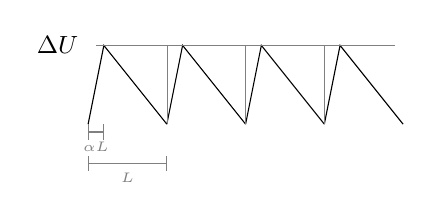
\begin{tikzpicture}
    \foreach \x in {0,1,2,3}
             {
               \draw (\x,0) -- ++(0.2, 1) -- ++(0.8, -1);
             }
    \draw[gray, very thin] (0.1, 0.001) grid (3.9, 1);
    \draw[|-|, gray, thin] (0,0) ++(0, -0.1) -- ++(0.2, 0) node[midway, anchor=north] {\tiny $\alpha L$};
    \draw[|-|, gray, thin] (0,0) ++(0, -0.5) -- ++(1, 0) node[midway, anchor=north] {\tiny $L$};
    \node[anchor=east] at (0, 1) {\small $\Delta U$};

  \end{tikzpicture}
  \caption{Ratchet potential. \label{fig:pot}}
\end{figure}

Assume that each particles may be treated independently.
The forces at play are those from the potential gradient, from friction, and the random walk term.
From Newton's second law this gives
\begin{equation}\label{eq:equation_of_motion}
m_i \dderiv{x_i}{t} =
-\del{U}{x} (x_i, t) - \gamma_i \deriv{x_i}{t} + \xi(t),
\end{equation}
where $\gamma_i = 6\pi \eta r_i$ is a friction constant and $\xi$ is a stochastic variable modeling the random walk.
The stochastic variable has a distribution such that
\begin{equation}
  \expval{\xi(t)} = 0, \quad \expval{\xi(t)\xi(t')} = 2\gamma_i k_B T \delta (t-t'),
\end{equation}
where $k_B$ is the Boltzmann constant and $T$ the temperature \cite{assignment}.

We remove the term with the second derivative, and rewrite as
\begin{equation}\label{eq:ode}
\gamma_i \deriv{x_i}{t} = -\del{U}{x}(x_i, t) + \xi(t)
\end{equation}


Due to the picewise linear nature of the potential, the forward Euler scheme is sufficient.
One thus gets \cite{assignment}
\begin{equation}\label{eq:euler}
x_{n+1} = x_n - \frac{1}{\gamma_i} \del{U}{x}(x_n, t_n) \delta t
+ \sqrt{\frac{2k_B T \delta t}{\gamma_i}} \hat{\xi}_n.
\end{equation}

The time step $\delta t$ must be chosen such that
$$
| x_{n+1} - x_n | \ll \alpha L.
$$
Notice that $\alpha L$ is the shortest piece of constant force from the potential, and this condition therefore ensures that the particle does not "skip" any parts of the potential.
Inserting this into \eqref{eq:euler} yields
\begin{equation}
\frac{1}{\gamma_i} \operatorname{max}\left| \del{U}{x} \right| \delta t + 4\sqrt{\frac{2k_B T \delta t}{\gamma_i}} \ll \alpha L,
\end{equation}
where we used the fact that $|\hat{\xi}_n|<4$ with 99.99\% probability.


We will use the Boltzmann distribution and diffusion equation to check numeric validity.
During the trapping phase, the particles should follow the Boltzmann distrubution for the potential.
When the potential is off, the particles should diffuse freely.

From \cite{assignment} one has the Boltzmann distrbution
\begin{equation}\label{eq:boltzmann}
p(U) =
\frac{
  e^{-\frac{U}{k_BT}}
}{
  k_BT \left(
  1 - e^{-\frac{\Delta U}{k_BT}}
  \right)
}.
\end{equation} and that the diffusion equation gives a particle distribution with a standard deviation proportional to the square root of time.

Introducing dimensionless quantities
\begin{equation}\label{eq:dimless}
\hat{x} = \frac{x}{L},\quad
\hat{t} = \omega t,\quad
\omega = \frac{\Delta U}{\gamma_i L^2},\quad
\hat{U}(\hat{x}, \hat{t}) = \frac{U(x, t)}{\Delta U},\quad
\hat{D} = \frac{k_BT}{\Delta U}
\end{equation}
the Euler scheme \eqref{eq:euler} may be written
\begin{equation}\label{eq:euler_dimless}
\hat{x}_{n+1} = \hat{x}_n - \del{\hat{U}}{\hat{x}}(\hat{x}, \hat{t})\delta \hat{t} + \sqrt{2\hat{D}\delta\hat{t}} \hat{\xi}_n.
\end{equation}
Notice that the particles radius only appears in $\omega$, through $\gamma$.
Changing particle size thus corresponds to simply scaling the time.

\section{Results and discussion}
In the following, the values from the original experiment were used, with thermal energy of \SI{26}{\milli\eV}, potential $\Delta U = \SI{80}{\eV}$, potential periodicity $L=\SI{20}{\micro\meter}$, and a diffusion constant of $\SI{1.8e-7}{\cm\squared\per\second}$.
Converting the bla bla bla, we deduce $r=\SI{12}{\nano\meter}$.

Firstly, to check the validity of the model the simulation was run with a constant ratchet potential.
Figure \ref{fig:traj} shows the trajectory of one particle.
In figure \ref{fig:boltzmann} the distribution of particles that have been allowd to diffuse in the time independent potential is shown for two different values of the diffusion constant, $D=0.1$ and $D = 0.2$.
Both figures indicate that the model performs well.
The distribution does follow the Boltzmann distrbution during the trapping phase.
From the trajectory one can see that the particle is biased towards the negative side of the potential well.
In figure \ref{fig:diffusion} the standard deviation $\sigma$ of an ensable of particles is shown.
As expected from theory, $\sigma \propto \sqrt{t}$.


\begin{figure}[ht]
\centering
\includegraphics[width=.75\textwidth]{media/diffusion}
\caption{The standard deviation of an ensable of particles and the square root of time.
\label{fig:diffusion}}
\end{figure}

\begin{figure}
\centering
\subcaptionbox{$D=\frac{1}{10}$}{\includegraphics[width=0.49\textwidth]{media/boltzmannD01}}
\subcaptionbox{$D=\frac{1}{5}$}{\includegraphics[width=0.49\textwidth]{media/boltzmannD02}}
\caption{The simulated distrubution in a time independent potential for $D=0.1$ and $D=0.2$.
The orange lines show the theoretial Boltzmann distribution.\label{fig:boltzmann}}
\end{figure}

\begin{figure}[ht]
\centering
\includegraphics[width=0.75\textwidth]{media/particle_trajectory}
\caption{Particle trajectory in time independent potential.
Notice that the position is not symmetric when trapped, but biased towards the negative end, due to the lower slope of the potential there.\label{fig:traj}}
\end{figure}


What remains is determining an optimal flashing period, $\tau_{op}$, that maximized the drift velocity and use this flashing period on two particles of different size, to see if one is able to separate them.
Figure \ref{fig:drift_vel} shows the average drift distance using different flashing periods.
For each flashing period, 500 realisations were made and the particles were simulated until $\hat{t} = 4000$.
With a particle of $r=\SI{12}{\nano\meter}$ the optimal flashing period is found to be 0.50s, or \SI{2.0}{\hertz}, giving a drift velocity of \SI{4.3}{\micro\meter\per\second}.
With a 1.4s period, the period used in the original experiment, the particle drifted $4.6L$ per 20 cycle, or \SI{3.3}{\micro\meter\per\second}.
This is in very good correspondence with the original experiment, where the particles drifted $5L$ in 20 cycles.

Changing the size of the particle corresponds to simply changing the friction constant $\gamma$, which in turn, according to \eqref{eq:dimless}, corresponds to scaling the time.
Considering a particle with radius $r_2 = 3r$ gives a new $\omega_2 = \omega/3$, thus
$$
\hat{t} = \omega_2 t_2 \Rightarrow t_2 = 3\frac{\hat{t}}{\omega} = 3t.
$$
Thus, using a flashing period optimized for the $r_2$ particle will only give a drift velocity of a third of that of the smaller particle.
Moreover, when using the flashing period optimized for the $r$ particle, this will be suboptimal for the $r_2$ particle.
The optimal drift velocity, in dimensionless units, is according to figure \ref{fig:drift_vel} is $\tau = 70$.
The bigger particle will experience a period of three times that, $\tau = 210$, which gives a total drift of $4.2L$.
Remembering that one also has to divide by three, as the bigger particle has experienced three times as much time, one gets $1.4L$, opposed to the smaller particle's $6.1L$.
The smaller particle has a drift velocity of 4.4 that of the bigger particle.
Figure \ref{fig:separation} shows the particle density where the two types of particles have been simulated for the same length of time with the flashing period optimized for the smaller particles.
From inspection, the calculated velocity difference of 4.4 is consistent with the difference in total travel for the two types of particles.




\begin{figure}[ht]
\centering
\includegraphics[width=.75\textwidth]{media/drift_dist}
\caption{Total drifted distance $x$ in units of periodicity length $L$ for different flashing periods $\tau$.
Particles allowed to drift for $4000$ time units.
Quantities presented in dimensionless units in order to apply the results to different values of $r$.
\label{fig:drift_vel}}
\end{figure}

\begin{figure}[ht]
\centering
\includegraphics[width=.75\textwidth]{media/particle_separation}
\caption{Separation of particles with different size.
The big partilces have three times the radius of the small partilces.
\label{fig:separation}}.
\end{figure}

\section{Conclusion}
Using a simple Langevin approach, solved with Forward Euler, one is able to recreate the same findings numerically as was found in the original experiment.
For the type of particle used in the experiment, the numerical approach found the optimal flashing period to be \SI{0.50}{s}, giving a drift velocity of \SI{4.3}{\micro\meter\per\second}.
With the flashing period used in the original experiment, we here found the drift velocity to be $4.6L$ per 20 cycle, in good correspondence with the original experiment's $5L$ per 20 cycle.
We also showed that one is able to get good separation of particles of different sizes.
With two particles, with one having three times the radius of ther other, the smaller particle was found to have a drift velocity of 4.4 that of the bigger particle.

\begin{thebibliography}{9}
\bibitem{assignment} Assignment

  \bibitem{experiment} Real experimetn
\end{thebibliography}
\end{document}
